% Full forward-modelling and inference workflow.
\documentclass[tikz,border=1pt]{standalone}
\usepackage{newtxtext,newtxmath}
\usepackage[T1]{fontenc}
\usepackage{amsmath}
\usetikzlibrary{arrows.meta,calc}
\graphicspath{{plots/}}

% ---------------------------------------------------------------- colours
\definecolor{eorc}{HTML}{1E3A6E}   % 21-cm signal (dark blue)
\definecolor{fgc}{HTML}{A3182F}    % foregrounds (crimson red)
\definecolor{instc}{HTML}{4A5568}  % instrument / data
\definecolor{infc}{HTML}{4A5568}   % inference (same neutral grey as instrument/data)
\colorlet{cubeedge}{white}
\colorlet{shadow}{black}
\colorlet{panelbg}{white}
\colorlet{ink}{black}
\ifdefined\DarkWorkflow
  \graphicspath{{\DarkPlots/}{plots/}}
  % Match Material's dark canvas while retaining the scientific image colours.
  \definecolor{canvas}{HTML}{1E2129}
  \definecolor{panelbg}{HTML}{242833}
  \definecolor{ink}{HTML}{E7EAF0}
  \definecolor{eorc}{HTML}{93ADDA}
  \definecolor{fgc}{HTML}{E55773}
  \definecolor{instc}{HTML}{A6B0C0}
  \colorlet{infc}{instc}
  \pagecolor{canvas}
  \AtBeginDocument{\color{ink}}
\fi

% ------------------------------------------------------------------ styles
\tikzset{
  panel/.style={draw=#1, fill=panelbg, line width=0.8pt,
                anchor=north west, inner sep=0pt},
  stage/.style={draw=instc, fill=panelbg, line width=0.6pt,
                anchor=north west, inner sep=0pt,
                minimum width=2.91cm, minimum height=2.45cm},
  ttl/.style={font=\footnotesize\bfseries, align=center},
  lbl/.style={font=\footnotesize, align=center},
  small/.style={font=\scriptsize, text=ink!70!panelbg, align=center},
  flow/.style={-{Stealth[length=2.4mm,width=2mm]}, line width=1.1pt, draw=#1},
  flow/.default=instc,
  op/.style={font=\small, text=#1},
  op/.default=ink,
  thumb/.style={inner sep=0pt},
}
\newcommand{\bm}[1]{\boldsymbol{#1}}
% \eorcube{x}{y}{size}{file prefix}: cube with front/top/side face images,
% lower-left corner of the front face at (x,y)
\newcommand{\eorcube}[4]{%
  \pgfmathsetmacro{\a}{#3}\pgfmathsetmacro{\dx}{0.38*#3}\pgfmathsetmacro{\dy}{0.265*#3}%
  \begin{scope}[shift={(#1,#2)}]
    \node[thumb, anchor=south west] at (0,0)
         {\includegraphics[width=\a cm,height=\a cm]{#4_front.png}};
    \begin{scope}[cm={1,0,\dx/\a,\dy/\a,(0,\a)}]
      \node[thumb, anchor=south west, transform shape] at (0,0)
           {\includegraphics[width=\a cm,height=\a cm]{#4_top.png}};
    \end{scope}
    \begin{scope}[cm={\dx/\a,\dy/\a,0,1,(\a,0)}]
      \node[thumb, anchor=south west, transform shape] at (0,0)
           {\includegraphics[width=\a cm,height=\a cm]{#4_side.png}};
    \end{scope}
    \draw[cubeedge, line width=0.4pt, line join=round]
         (0,0) -- (\a,0) -- (\a,\a) -- (0,\a) -- cycle
         (0,\a) -- (\dx,\a+\dy) -- (\a+\dx,\a+\dy) -- (\a,\a)
         (\a+\dx,\a+\dy) -- (\a+\dx,\dy) -- (\a,0);
  \end{scope}}


\begin{document}
\begin{tikzpicture}[x=1cm,y=1cm]

% Column grid (cm): five equal 2.91 cm columns, 0.6 cm gutters (0.65 before R)
%   c1 0.45-3.36 | c2 3.96-6.87 | c3 7.47-10.38 | c4 10.98-13.89 | R 14.54-17.45
%   centres: 1.905 | 5.415 | 8.925 | 12.435 | 15.995
% Rows (all boxes 2.45 cm tall):
%   row 1  -0.07 .. -2.52   (Model Parameters outline 0.01 .. -2.60; drawn with yshift)
%   row 2  -3.52 .. -5.97   (Forward Model outline   -3.44 .. -6.05; equation below at -6.43)
%   row 3  -6.90 .. -9.35   (Inference L-outline, arm -6.82 .. -9.43)
% Outline labels sit on the left edge of each dashed outline, reading upwards.
\tikzset{grouplabel/.style={fill=panelbg, draw=instc, font=\footnotesize\bfseries,
                            inner xsep=3pt, inner ysep=2pt, rotate=90}}
% =====================================================================
%  ROW 1 : 21-cm model (c1+c2), foreground model (c3+c4), data (R)
% =====================================================================
\begin{scope}[yshift=0.15cm]   % row 1 sits 0.15 cm higher to leave room for the Q_z label
\draw[instc, dashed, line width=0.7pt] (0.2,-0.14) rectangle (13.97,-2.75);
\node[grouplabel] at (0.2,-1.445) {Model Parameters};

% ---- Fourier-domain 21-cm model -----------------------------------------
\node[panel=eorc, fill=eorc!12!panelbg, minimum width=6.42cm, minimum height=2.45cm] (eor) at (0.45,-0.22) {};
\node[ttl] at (3.66,-0.50) {Fourier-Domain 21-cm Model};
\node[lbl] at (3.66,-0.84) {$\bm{a}(u,v,\eta)$};
% three cubes: the same 21-cm realisation band-passed into low / mid / high
% spherical k shells, drawn with increasing size (k_1 < k_2 < k_3)
\eorcube{1.68}{-2.30}{0.55}{eor_k1}
\eorcube{2.84}{-2.30}{0.76}{eor_k2}
\eorcube{4.29}{-2.30}{0.98}{eor_k3}
\node[small, text=eorc] at (1.955,-2.45) {$k_1$};
\node[small, text=eorc] at (3.22,-2.45) {$k_2$};
\node[small, text=eorc] at (4.78,-2.45) {$k_3$};

% ---- image-domain foreground model ---------------------------------------
\node[panel=fgc, fill=fgc!12!panelbg, minimum width=6.42cm, minimum height=2.45cm] (fg) at (7.47,-0.22) {};
\node[ttl] at (10.68,-0.50) {Image-Domain Foreground Model};
\node[lbl] at (10.68,-0.84) {$\bm{q}(l,m,n)$};
% spectral-basis maps: overlapping stack of "plates" (back -> front)
\foreach \f/\lab/\k in {fg_q0/q_0/0, fg_q1/q_1/1, fg_q2/q_2/2}{
  \pgfmathsetmacro{\yc}{-1.45-0.36*\k}
  \fill[shadow, opacity=0.22] (10.70,\yc-0.05) ellipse (1.30 and 0.39);
  \node[thumb] at (10.68,\yc) {\includegraphics[width=2.6cm,height=0.78cm]{\f.png}};
  \node[small, text=ink!80!panelbg, anchor=west] at (12.10,\yc) {$\lab$};
}

% ---- data ----------------------------------------------------------------
\node[panel=instc, minimum width=2.91cm, minimum height=2.45cm] (data) at (14.54,-0.22) {};
\node[ttl] at (15.995,-0.50) {Observed Data};
\node[lbl] at (15.995,-0.84) {$\bm{d}(\bm{b}_{ij},\nu,t)$};
\node[thumb] at (15.995,-1.78) {
\includegraphics{icon_array.pdf}};   % HERA-37 layout
\end{scope}

% =====================================================================
%  ROW 2 : forward model  ->  full likelihood
% =====================================================================
\draw[instc, dashed, line width=0.7pt] (0.2,-3.44) rectangle (13.97,-6.05);
\node[grouplabel] at (0.2,-4.745) {Forward Model};

\node[stage] (b1) at (0.45,-3.52) {};
\node[stage] (b2) at (3.96,-3.52) {};
\node[stage] (b3) at (7.47,-3.52) {};
\node[stage] (b4) at (10.98,-3.52) {};
\foreach \b/\t/\m/\img in {
  b1/{Sky Fourier Space}/{$S(u,v,\nu)$}/sky_fourier,
  b2/{Sky Image Space}/{$I(l,m,\nu,t)$}/sky_image,
  b3/{Primary Beam}/{$P(l,m,\nu)\,I(l,m,\nu,t)$}/sky_beam,
  b4/{Sampled Visibilities}/{$V(\bm{b}_{ij},\nu,t)$}/visibilities}{
  \node[ttl, font=\scriptsize\bfseries] at ($(\b.north)+(0,-0.25)$) {\t};
  \node[small, text=ink] at ($(\b.north)+(0,-0.55)$) {\m};
  \node[thumb] at ($(\b.north)+(0,-1.55)$) {\includegraphics[width=1.60cm]{\img.png}};
}
\draw[flow=eorc] (b1.east) -- node[above, op=eorc] {$\mathbf{F}'$} (b2.west);
\draw[flow]      (b2.east) -- node[above, op] {$\mathbf{P}$} (b3.west);
\draw[flow]      (b3.east) -- node[above, op] {$\mathbf{F}^{-1}$} (b4.west);

% component inputs: 21-cm enters in Fourier space, foregrounds in image space
\draw[flow=eorc] (1.905,-2.52) -- node[right, op=eorc, pos=0.45] {$\mathbf{F}_z$} (1.905,-3.52);
\draw[flow=fgc] (8.1,-2.52) -- (8.1,-2.90) -- (5.415,-2.90) -- (5.415,-3.52);
\node[op=fgc, anchor=west, inner sep=1pt] at (5.465,-3.11) {$\mathbf{Q}_z$};

% the one equation (between the Forward Model and Inference outlines)
\node[font=\small] at (7.08,-6.43)
  {$\bm{m}=\mathbf{F}^{-1}\mathbf{P}\big(\textcolor{eorc}{\mathbf{F}'\mathbf{F}_z\bm{a}}
   +\textcolor{fgc}{\mathbf{Q}_z\bm{q}}\big)$};

% =====================================================================
%  MARGINALISED INFERENCE : L-shaped outline (data, likelihood, row 3)
% =====================================================================
\draw[instc, dashed, line width=0.7pt]
  (14.46,0.01) -- (17.53,0.01) -- (17.53,-9.43) -- (0.2,-9.43) -- (0.2,-6.82)
  -- (14.46,-6.82) -- cycle;
\node[grouplabel] at (0.2,-8.125) {Inference};

% ---- full likelihood: data vs model visibility waterfalls (nu x t) -------
\node[panel=instc, minimum width=2.91cm, minimum height=2.45cm] (like) at (14.54,-3.52) {};
\node[ttl] at (15.995,-3.77) {Full Likelihood};
\node[lbl] at (15.995,-4.11) {$\mathcal{L}(\bm{d}\mid\textcolor{eorc}{\bm{a}},\textcolor{fgc}{\bm{q}})$};
\node[thumb] at (15.995,-5.05) {
\includegraphics{icon_likelihood.pdf}};
\node[font=\scriptsize, text=instc] at (15.385,-5.69) {$\bm{d}$};
\node[font=\scriptsize] at (16.605,-5.69) {$\bm{m}$};
\draw[flow] (b4.east) -- (like.west |- b4.east);
\draw[flow] (data.south) -- (data.south |- like.north);

% =====================================================================
%  ROW 3 : full likelihood -> prior covariance -> marginalised likelihood
%          -> nested sampling -> outputs   (right to left)
% =====================================================================
% ---- parameterised prior covariance (R) ------------------------------------
\node[panel=infc, minimum width=2.91cm, minimum height=2.45cm] (prior) at (14.54,-6.90) {};
\node[ttl, anchor=north] at (15.995,-7.02) {Prior\\Covariance\ \mdseries\,$\mathbf{\Psi}(\bm{\varphi})$};
\node[thumb] at (16.045,-8.60) {
\includegraphics{icon_prior.pdf}};   % block-diagonal Psi
\node[small, text=eorc, anchor=east] at (15.30,-8.40) {$\mathbf{\Phi}(\bm{\varphi})$};
\node[small, text=fgc,  anchor=west] at (16.80,-9.02) {$\mathbf{\Sigma}_q$};
\draw[flow] (like.south) -- (prior.north);

% ---- marginalised likelihood (c4) ------------------------------------------
\node[panel=infc, minimum width=2.91cm, minimum height=2.45cm] (marg) at (10.98,-6.90) {};
\node[ttl, anchor=north] at (12.435,-7.02) {Marginalised\\Likelihood\ \mdseries\,$\mathcal{L}(\bm{d}\mid\bm{\varphi})$};
\node[thumb] at (12.435,-8.55) {
\includegraphics{icon_marginal.pdf}};
\draw[flow=infc] (prior.west) -- (marg.east |- prior.west);

% ---- nested sampling (c3) ---------------------------------------------------
\node[panel=infc, minimum width=2.91cm, minimum height=2.45cm] (ns) at (7.47,-6.90) {};
\node[ttl, anchor=north] at (8.925,-7.02) {Nested\\Sampling\ \mdseries\,$\bm{\varphi}$};
\node[thumb] at (8.925,-8.55) {
\includegraphics{icon_nested.pdf}};
\draw[flow=infc] (marg.west) -- (ns.east |- marg.west);

% ---- outputs (c1+c2) -----------------------------------------------------------
\node[panel=infc, minimum width=6.42cm, minimum height=2.45cm] (out) at (0.45,-6.90) {};
\draw[infc!45, dashed, line width=0.5pt] (3.66,-7.10) -- (3.66,-9.15);
\draw[flow=infc] (ns.west) -- (out.east |- ns.west);

% power spectrum
\node[ttl, anchor=north] at (2.055,-7.02) {Power Spectrum\ \mdseries\,$\Delta^2(k)$};
\node[thumb] at (2.055,-8.37) {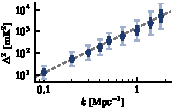
\includegraphics{icon_powerspec.pdf}};

% evidence
\node[ttl, anchor=north] at (5.265,-7.02) {Bayesian Evidence\ \mdseries\,$\mathcal{Z}$};
\node[thumb, anchor=south] at (5.265,-8.9785) {
\includegraphics{icon_evidence.pdf}};
\node[font=\scriptsize, text=eorc, anchor=north] at (4.695,-8.98) {$\mathcal{Z}_{\rm 21+FGs}$};
\node[font=\scriptsize, text=fgc,  anchor=north] at (5.835,-8.98) {$\mathcal{Z}_{\rm FG}$};

\end{tikzpicture}
\end{document}
